\documentclass[11pt,a4paper]{article}
\usepackage[margin=21mm]{geometry}
\usepackage{graphicx,booktabs,tabularx,array,amsmath,hyperref,float}
\hypersetup{colorlinks=true,linkcolor=blue,urlcolor=blue,pdftitle={Retained EEG quality and matched ErrP comparisons},pdfauthor={Satyam Awasthi}}
\setlength{\parindent}{0pt}\setlength{\parskip}{5pt}\sloppy
\newcommand{\uv}{\ensuremath{\mu\mathrm{V}}}
\newcommand{\reviewbox}{\par\vspace{3mm}\fbox{\parbox{.95\linewidth}{\textbf{Reviewer notes (optional)}\\[3mm]Suspected source / confidence: \hrulefill\\[5mm]Response overlap / recommended handling: \hrulefill\\[7mm]\mbox{}\hrulefill\\[7mm]\mbox{}\hrulefill}}}
\title{Retained EEG quality and matched ErrP comparisons\\\large A two-participant FORCe integration pilot}
\author{Satyam Awasthi}\date{}
\begin{document}\maketitle
\begin{abstract}
We linked input-quality flags to final trial decisions, screened retained EEG and compared matched event-related waveforms in two participants. All 180 inputs exceeding 1 mV were rejected by every processing condition. Smaller local or broad changes remained in selected accepted outputs, including inputs not previously flagged. Split-filter FORCe produced fewer output-screen flags and sharp joins, but both FORCe variants changed matched Error--Correct waveforms. Median waveform-change RMS was 2.04 and 2.81 \uv\ for the FORCe/control contrasts, versus 0.11 \uv\ between no-FORCe controls. These descriptive findings support a no-FORCe working analysis with targeted review and FORCe sensitivity comparisons; they do not establish artifact-source identities or neural-signal preservation.
\end{abstract}
\section{Question and processing design}
The question is whether existing quality-control and rejection adequately handle concerning inputs, and whether FORCe materially changes the error-related EEG findings. This note follows the input-contamination and boundary studies. It evaluates the tested integrations, rather than claiming an exact reproduction of the Graz preprocessing \cite{graz} or a general benchmark of FORCe \cite{force}.

The pilot comprises 29 selected recordings from mle01 and spe30 across pre, post and retest sessions. All eight EEG channels are included: P3, PO3, PO7, CP5, CP1, Cz, FCz and FC1. Of 2,915 trial rows, 2,799 have complete valid three-second inputs after event, loss/gap and recording-edge checks. The existing outputs are used throughout; no new FORCe tuning or rejection policy is applied.
\begin{table}[H]\centering\small
\begin{tabularx}{\linewidth}{@{}clX@{}}\toprule
ID & Processing condition & Sequence before common crop/baseline\\\midrule
1 & BP no-FORCe & Continuous 1--20 Hz bandpass; no cleaning.\\[3pt]
2 & BP FORCe & Same bandpass; clean three separate one-second windows.\\[3pt]
3 & Split no-FORCe & Continuous 1 Hz high-pass; 20 Hz low-pass over the three-second segment.\\[3pt]
4 & Split FORCe & Same high-pass; clean three one-second windows; low-pass over the rejoined segment.\\\bottomrule
\end{tabularx}
\caption{Processing IDs are consistent across tables and figures. BP denotes bandpass. Filters use nominal fourth-order Butterworth designs with forward--backward application.}\label{tab:conditions}
\end{table}
All conditions use movement marker 400 at $t=0$, inputs $[-1.5,1.5)$ s, crop $[-1,1)$ s, baseline subtraction over $[-0.2,0)$ s and final rejection when any channel exceeds 100 \uv\ in absolute value. FORCe still processes one-second windows, with internal joins at $-0.5$ and $+0.5$ s. Three seconds provide context and filtering padding, not a three-second FORCe call. Filtering is held constant within each FORCe/control pair. Cross-family comparisons evaluate practical pipelines, not filtering order alone.
\clearpage
\section{Measurements and interpretation}
\subsection{Linking input flags to trial decisions}
Trials are matched by recording identifier and original trial number. Input screens use continuously 1 Hz high-pass-filtered EEG before FORCe and the final low-pass, measured within three separate one-second windows. Slow and higher-frequency features are band RMS over 1--4 Hz and 30--90 Hz, excluding 48--52 Hz from the latter. A local-abrupt feature uses the largest absolute adjacent-sample change and requires channel range at least three times the median across channels.

Modified z-scores on log features flag unusually large slow, HF or step features ($z>3.5$). Each input reference uses participant, session, channel and window position. Other input screens identify absolute voltage above 100 \uv, 49--51 Hz power above 25\% of 1--90 Hz power, and gross excursions above 1 mV. These overlapping flags are inspection aids, not automatic source labels. Every flag is linked to acceptance or the saved rejection/precheck reason. The 116 unavailable inputs have no screens.
\subsection{Screening final retained signals}
Output measurements use the same baseline-corrected two-second interval in every condition. One-sided Hann-periodogram power spectral density (PSD) gives band RMS:
\[
f_{\mathrm{band}}=\sqrt{\sum_{k\in\mathrm{band}}\mathrm{PSD}[k]\,\Delta f},\qquad\Delta f=0.5\ \mathrm{Hz}.
\]
Output slow-band RMS, full voltage range and maximum adjacent-sample change are scored relative to \emph{accepted condition-1 outputs}, separately by participant, session and channel. This reference is held fixed for all conditions:
\[
z_{f,i}=0.67448975\frac{\log_{10}f_i-\operatorname{median}(\log_{10}f)}{\operatorname{MAD}(\log_{10}f)}.
\]
MAD is the median absolute deviation about the median. The 3.5 convention follows modified-z-score outlier labelling \cite{nist}; it is not an EEG-specific diagnostic threshold. Only the upper tail is screened. A local-abrupt output flag also requires the threefold spatial-range criterion. The combined output-review flag is the union of slow, range and local flags.

A separate join inspection flag requires either join's sample change to exceed three times that channel/trial's ordinary-change 95th percentile. Ordinary changes exclude 50 ms around $-0.5$, 0 and $+0.5$ s. This arbitrary inspection ratio is reported separately. Introduced joins remain part of the analysed signal. Genuine neural activity can meet the output rules; a relative reference can also miss persistent contamination.
\subsection{Matched event-related waveforms}
Correct means non-displaced (ND, label 1), Error means displaced (D, label 2), and Error--Correct means D minus ND. These labels do not establish an error percept on each trial. All conditions share the same 2,562 trials accepted by every condition. Means pool runs within participant/session with equal weight per trial. The main response interval is $T=[0.4,0.8)$ s; $[0.2,0.9)$ s is retained for broader descriptive comparison.

We measure signed mean amplitude, RMS, positive/negative extrema and times, and the signed largest-absolute extremum and time. For waveforms $d_a,d_b$:
\[
\Delta\bar d=\operatorname{mean}_{t\in T}[d_a(t)-d_b(t)],\quad
\mathrm{RMS}_{\Delta}=\sqrt{\operatorname{mean}_{t\in T}\{[d_a(t)-d_b(t)]^2\}}.
\]
Peak times are descriptive extrema, not validated component latencies. A changed extremum can mean selection of another peak rather than a physiological delay.
\clearpage
\section{Input flags and final retention}
There are 268 input-flagged mle01 trials and 98 input-flagged spe30 trials, using the union of all input screens. All 180 gross inputs above 1 mV occur in mle01 and are rejected by every condition. All 41 line-frequency-flagged inputs are also rejected in every condition. This concerns rejection, not recovery of corrupted EEG.
\begin{table}[H]\centering\small
\begin{tabular}{@{}lrrrrrr@{}}\toprule
Participant & ID & Eligible & Accepted ND & Accepted D & Total & Input-flagged\\\midrule
mle01 & 1 & 1411 & 766 & 413 & 1179 & 38 \\
mle01 & 2 & 1411 & 786 & 415 & 1201 & 58 \\
mle01 & 3 & 1411 & 767 & 415 & 1182 & 41 \\
mle01 & 4 & 1411 & 787 & 416 & 1203 & 60 \\
spe30 & 1 & 1388 & 915 & 471 & 1386 & 96 \\
spe30 & 2 & 1388 & 916 & 471 & 1387 & 97 \\
spe30 & 3 & 1388 & 915 & 471 & 1386 & 96 \\
spe30 & 4 & 1388 & 916 & 471 & 1387 & 97 \\
\bottomrule\end{tabular}
\caption{Condition-specific accepted sets. The last column counts retained inputs with a flag, not confirmed residual artifacts. ND/D denote non-displaced/displaced trials.}\label{tab:retention}
\end{table}
Without FORCe, eligible-trial rejection is by final amplitude: 232/1,411 mle01 and 2/1,388 spe30 trials in condition 1, versus 229 and two in condition 3. Condition 2 excludes 209 mle01 and one spe30 input by saved channel-threshold prechecks, plus one mle01 output by amplitude. Condition 4 excludes 208 and one by those prechecks. No final waveform after a precheck means unavailable output, not a zero or successfully cleaned signal.

The no-FORCe conditions disagree on only three of 2,799 eligible decisions: additional mle01 acceptances in condition 3. Conditions 1 versus 2 have 2,562 trials accepted by both, 26 only with FORCe, three only without and 208 rejected by both. More retained input flags after FORCe do not imply worse cleaning: attenuation can allow a flagged input to meet the amplitude rule.
\subsection{Filtering can address an input feature}
For 31 retained spe30 HF-flagged trials, median matched-channel HF RMS ratios are 0.00671 for condition 1 versus HP-only input and 0.00853 for condition 3, corresponding to about 99.3\% and 99.1\% RMS attenuation. Measurements use identical two-second samples and originally flagged channels. This is expected suppression by analysis filtering, not a percentage of artifacts removed or evidence of FORCe benefit.

For four retained mle01 local-input flags, median largest-step ratios after either no-FORCe filtering scheme are approximately 0.04 of matched HP input. A broad P3 deflection nevertheless remains in a reviewed trial. Attenuation of a sharp change does not guarantee disappearance of a broader disturbance.
\subsection{Denominators and review coverage}
Retention and quality tables use each condition's own accepted set. The ERP comparison instead uses the four-condition intersection, removing selection differences but omitting trials accepted by only some methods. Fourteen retained-trial examples were visually screened: targeted candidates, processing-related changes and one randomly selected input-unflagged accepted trial per participant/session (six total). This is an initial computational/visual assessment, not independent expert identification or a prevalence estimate.
\clearpage
\section{Residual quality in accepted EEG}
\begin{table}[H]\centering\small
\begin{tabular}{@{}lrrrrrrr@{}}\toprule
Participant & ID & Accepted & Slow & Range & Local & Any & Join\\\midrule
mle01 & 1 & 1179 & 27 & 43 & 4 & 50 & 0 \\
mle01 & 2 & 1201 & 15 & 18 & 40 & 63 & 797 \\
mle01 & 3 & 1182 & 26 & 43 & 4 & 50 & 0 \\
mle01 & 4 & 1203 & 10 & 2 & 0 & 12 & 6 \\
spe30 & 1 & 1386 & 4 & 44 & 0 & 47 & 0 \\
spe30 & 2 & 1387 & 0 & 14 & 0 & 14 & 1020 \\
spe30 & 3 & 1386 & 4 & 43 & 0 & 46 & 0 \\
spe30 & 4 & 1387 & 0 & 0 & 0 & 0 & 7 \\
\bottomrule\end{tabular}
\caption{Final-output flags across each condition's accepted set. Any is the union of Slow, Range and Local; categories overlap. Join is the separate boundary inspection flag, excluded from Any. These are feature counts, not confirmed artifact prevalence.}\label{tab:quality}
\end{table}
\begin{table}[H]\centering
\begin{tabular}{@{}lrrrr@{}}\toprule
Participant & Condition 1 & Condition 2 & Condition 3 & Condition 4\\\midrule
mle01 & 21/38 & 22/58 & 22/41 & 6/60 \\
spe30 & 8/96 & 4/97 & 8/96 & 0/97 \\
\bottomrule\end{tabular}
\caption{Retained input-flagged trials meeting an output-review rule / all retained input-flagged trials. Absence of an output flag does not certify removal: input and output screens use different durations and references.}\label{tab:followup}
\end{table}
Conditions 1 and 3 reject gross inputs but retain some smaller/local changes. In condition 1, 21 of 38 retained input-flagged mle01 trials and eight of 96 spe30 trials meet output-review criteria. Another 29 mle01 and 39 spe30 accepted trials are output-flagged despite no input flag. Reviewing only input-flagged trials would miss these candidates.

Appendix~\ref{app:examples} illustrates the distinction. Mle01 post run 4 trial 40 retains a broad P3-local deflection in both no-FORCe outputs; both FORCe prechecks exclude it. Mle01 post run 3 trial 82 is input-unflagged but has a substantial P3-local waveform in accepted controls. Spe30 retest run 5 trial 80 has an input-unflagged CP5-local change around $+0.4$ s, leaving a broad transition within the response interval. Source attribution and whether exclusion is justified remain open.

In mle01 pre run 1 trial 70, condition 2 has a CP1 adjacent-sample step of 6.079 \uv\ exactly at the $+0.5$ s join. Across matched accepted pairs, condition 2 introduces 33 new combined output-review candidates in mle01 and one in spe30 relative to condition 1. These feature changes do not independently establish neural damage.

Condition 4 has fewer output-review and join flags. Zero combined flags in spe30 condition 4 means only that tested features no longer exceed the fixed-reference thresholds; it does not establish artifact-free or response-preserving EEG. Lower scores may reflect useful cleaning, attenuation of relevant activity, or both.
\clearpage
\section{Matched ErrP waveform changes}
The common set contains 475/332/369 mle01 trials and 495/498/393 spe30 trials in pre/post/retest (2,562 total). Appendix~\ref{app:erp} shows all eight channels' Correct, Error and Error--Correct waveforms with class counts, onset and cleaning joins.
\begin{table}[H]\centering\small
\begin{tabular}{@{}lrrrr@{}}\toprule
Contrast & Median $|\Delta\bar d|$ & Max $|\Delta\bar d|$ & Median $\mathrm{RMS}_{\Delta}$ & Median $|\Delta t_{\min}|$\\
 & (\uv) & (\uv) & (\uv) & (ms)\\\midrule
2 minus 1 & 0.808 & 3.590 & 2.042 & 7 \\
4 minus 3 & 0.792 & 4.252 & 2.811 & 10 \\
3 minus 1 & 0.104 & 0.238 & 0.108 & 0 \\
4 minus 2 & 0.226 & 0.510 & 0.836 & 6 \\
\bottomrule\end{tabular}
\caption{Error--Correct changes over 0.4--0.8 s. Each row summarises 48 channel/session comparisons (eight channels, six participant/session means), not independent participant replicates or population significance tests. $t_{\min}$ is the most negative sample's time.}\label{tab:erpchanges}
\end{table}
The no-FORCe conditions are close: median absolute mean-amplitude change is 0.104 \uv\ and median waveform-change RMS is 0.108 \uv. Adding FORCe gives median absolute mean changes of 0.808 and 0.792 \uv\ for the bandpass and split pairs, with RMS changes of 2.042 and 2.811 \uv. The split integration's lower output-screen counts therefore do not imply smaller matched waveform changes.
\begin{table}[H]\centering\small
\begin{tabular}{@{}llrrrr@{}}\toprule
Participant & Session & Condition 1 & Condition 2 & Condition 3 & Condition 4\\\midrule
mle01 & pre & -0.660 & -0.451 & -0.517 & -0.454 \\
mle01 & post & -1.206 & -0.165 & -0.999 & +0.153 \\
mle01 & retest & -1.965 & -0.260 & -1.812 & -0.633 \\
spe30 & pre & +1.859 & -1.654 & +2.006 & -2.164 \\
spe30 & post & +0.898 & -1.195 & +1.039 & -1.622 \\
spe30 & retest & -1.040 & -1.417 & -0.914 & -1.253 \\
\bottomrule\end{tabular}
\caption{FCz mean Error--Correct amplitude (\uv) over 0.4--0.8 s, with identical trials across columns. A change in the window mean's sign is not a validated ERP component reversing polarity.}\label{tab:fcz}
\end{table}
In spe30 pre, FCz mean Error--Correct changes from $+1.859$ to $-1.654$ \uv\ with bandpass FORCe, and from $+2.006$ to $-2.164$ \uv\ with split FORCe. Post-session means also change sign in both pairs. These changes can affect interpretation and are not explained by different retained-trial IDs here.

Median absolute negative-extremum time changes are seven and ten milliseconds for the FORCe/control contrasts, but maxima reach 314 and 312 ms. Even the small filter-only contrast can select a different extremum. These are not established physiological delays: competing peaks, interval-edge selection, polarity and joins can affect the selected sample.
\clearpage
\section{Conclusions and limits}
\textbf{No-FORCe quality control rejects the gross pilot disturbances, but does not certify all accepted trials as clean.} Selected smaller/local waveforms remain; some were not input-flagged. Targeted expert assessment is warranted before treating those candidates as artifacts or applying new exclusions.

\textbf{Split filtering without FORCe produces similar screening counts and matched averages to bandpass no-FORCe.} It retains three additional inputs and gives small average-waveform differences. This is evidence about the tested implementations, not formal equivalence.

\textbf{Split FORCe produces fewer tested outliers and sharp joins than bandpass-before-FORCe.} This strengthens its case relative to that particular integration, but does not validate neural preservation or general superiority. Both variants substantially change some matched Error--Correct waveforms, including response-window mean signs.

\textbf{The evidence supports no-FORCe as the primary working analysis with targeted review, and FORCe as a secondary sensitivity analysis.} This does not establish that cleaning is unnecessary for every participant or that all FORCe changes are harmful. The pilot establishes that processing affects the findings, not which waveform is the uncontaminated neural response.
\subsection{Limits}
Only two participants were examined. Trial counts increase within-participant coverage, not independent cohort replication. Sources were not independently labelled; there are no EOG/EMG reference channels. The initial visual assessment is not blinded expert validation. Relative scores can flag genuine responses or miss persistent contamination.

The ERP intersection isolates waveform changes but does not assess the benefit of each method's additional accepted trials. Classification, population inference and canonical component identification are outside this note. The results do not by themselves explain unexpected ErrP timing or sign.
\subsection{Checks and accompanying material}
All 2,799 screened IDs match saved decisions, labels and eligibility. Common ERP samples are finite, meet saved amplitude acceptance and have baseline means within numerical tolerance. Broader-window Cz/FCz metrics reproduce the preceding saved analysis to $10^{-10}$ tolerance. Summaries preserve participant/session/run and displaced/non-displaced separation. Exact matched IDs, feature tables and the complete 14-example review set are retained with the analysis. Earlier reports and production settings were not changed to prepare this note.
\clearpage\appendix
\section{References}
\begin{thebibliography}{9}
\bibitem{graz} I. Amaunam, M. Sultana, B. Rodriguez-Herreros, T. Tadi, R. Leeb and S. Perdikis (2024). EEG correlates of error-related activity during ballistic computer mouse movements. \textit{9th Graz BCI Conference}. \href{https://repository.essex.ac.uk/38379/1/tDCS_ErrP_9th_Graz_BCI_Conference_2024.pdf}{University of Essex repository}.
\bibitem{force} I. Daly, R. Scherer, M. Billinger and G. M\"uller-Putz (2015). FORCe: Fully Online and Automated Artifact Removal for Brain-Computer Interfacing. \textit{IEEE Transactions on Neural Systems and Rehabilitation Engineering}, 23(5), 725--736. \href{https://doi.org/10.1109/TNSRE.2014.2346621}{doi:10.1109/TNSRE.2014.2346621}.
\bibitem{nist} NIST/SEMATECH. \textit{e-Handbook of Statistical Methods}, Section 1.3.5.17: Detection of Outliers. \url{https://www.itl.nist.gov/div898/handbook/eda/section3/eda35h.htm}.
\end{thebibliography}
\clearpage
\section{Focused retained-trial examples}\label{app:examples}
These are initial observations, not independent artifact labels. The complete review covered 14 trials, including six random input-unflagged accepted trials. Positive voltage is upward; no-FORCe is dashed and FORCe solid. Panels show a selected local channel and FCz. Writing space is provided for expert assessment.
\subsection*{B.1 A retained P3-local broad change}
\textbf{mle01 / post / run 4 / trial 40}

Both no-FORCe outputs pass amplitude rejection while retaining a broad P3-local deflection. Both FORCe prechecks exclude the input, so no cleaned final waveforms are available. Is this unacceptable contamination, and is trial or surrounding-data exclusion warranted?
\begin{figure}[H]\centering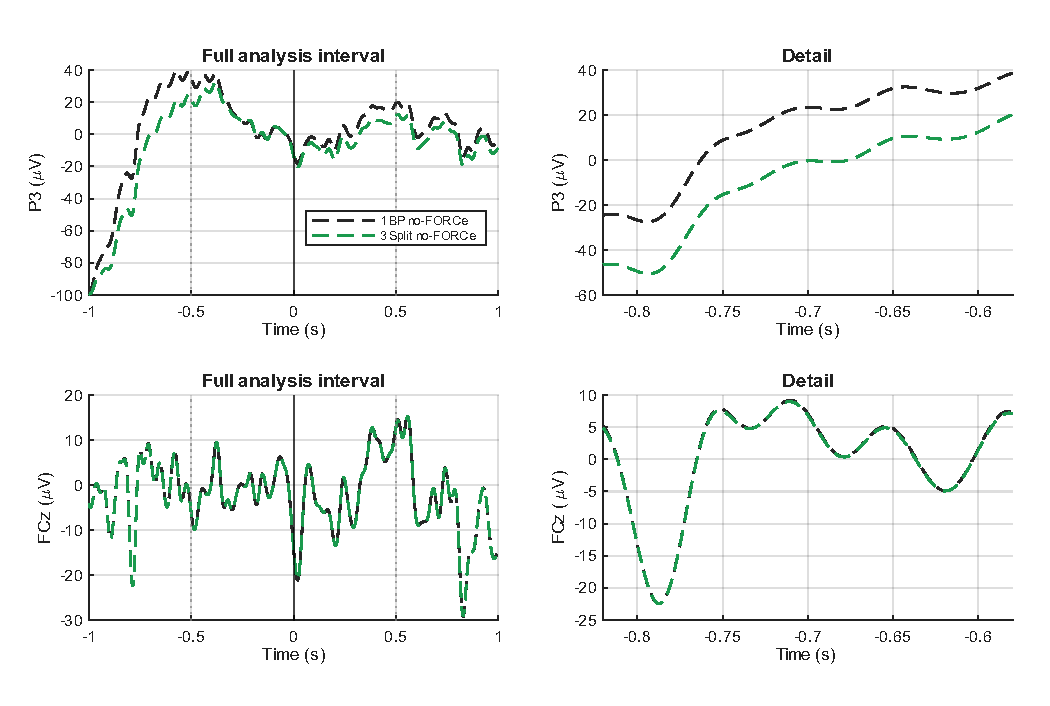
\includegraphics[width=\linewidth,height=.45\textheight,keepaspectratio]{figures/priority_1.pdf}\caption{Final outputs for mle01 / post / run 4 / trial 40. Conditions follow Table~\ref{tab:conditions}; onset is black and cleaning joins grey dotted.}\end{figure}
\reviewbox
\clearpage
\subsection*{B.2 An input-unflagged retained local waveform}
\textbf{mle01 / post / run 3 / trial 82}

All conditions accept this trial. P3-local excursions remain in the controls below 100 microvolts. FORCe attenuates them but also changes other channels. The input screen did not flag this trial; source and appropriate handling require review.
\begin{figure}[H]\centering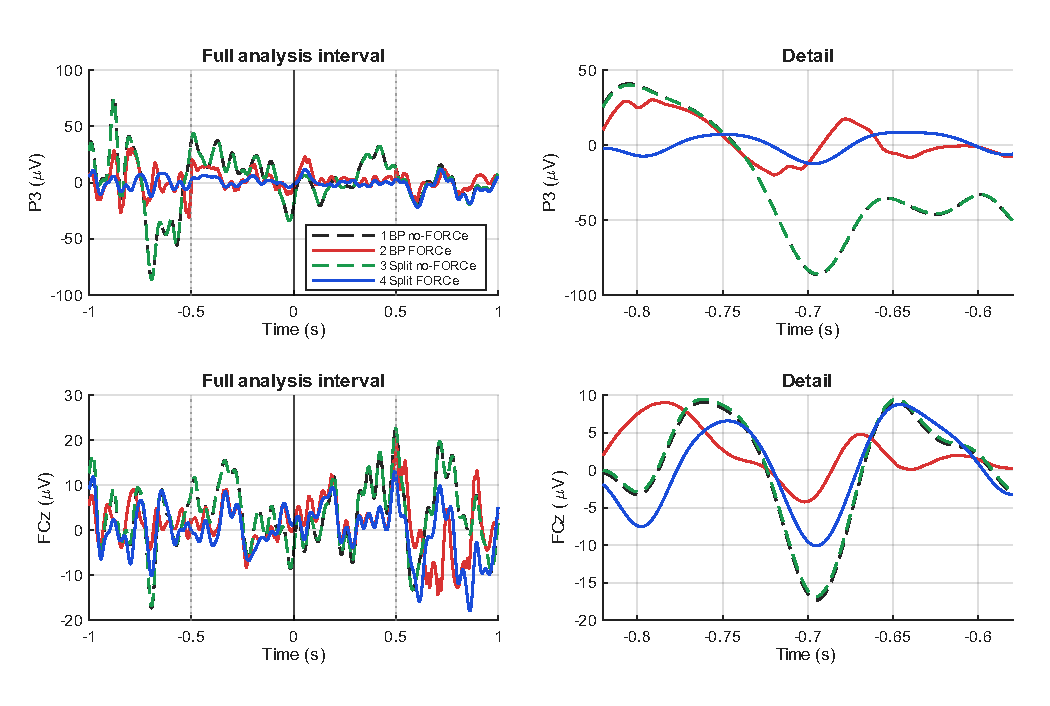
\includegraphics[width=\linewidth,height=.45\textheight,keepaspectratio]{figures/priority_2.pdf}\caption{Final outputs for mle01 / post / run 3 / trial 82. Conditions follow Table~\ref{tab:conditions}; onset is black and cleaning joins grey dotted.}\end{figure}
\reviewbox
\clearpage
\subsection*{B.3 A response-region CP5-local change}
\textbf{spe30 / retest / run 5 / trial 80}

All conditions accept this input-unflagged trial. A CP5-local change around +0.4 s becomes a broad transition within the response interval in both no-FORCe outputs. FORCe substantially changes it. Is its morphology consistent with a recording disturbance?
\begin{figure}[H]\centering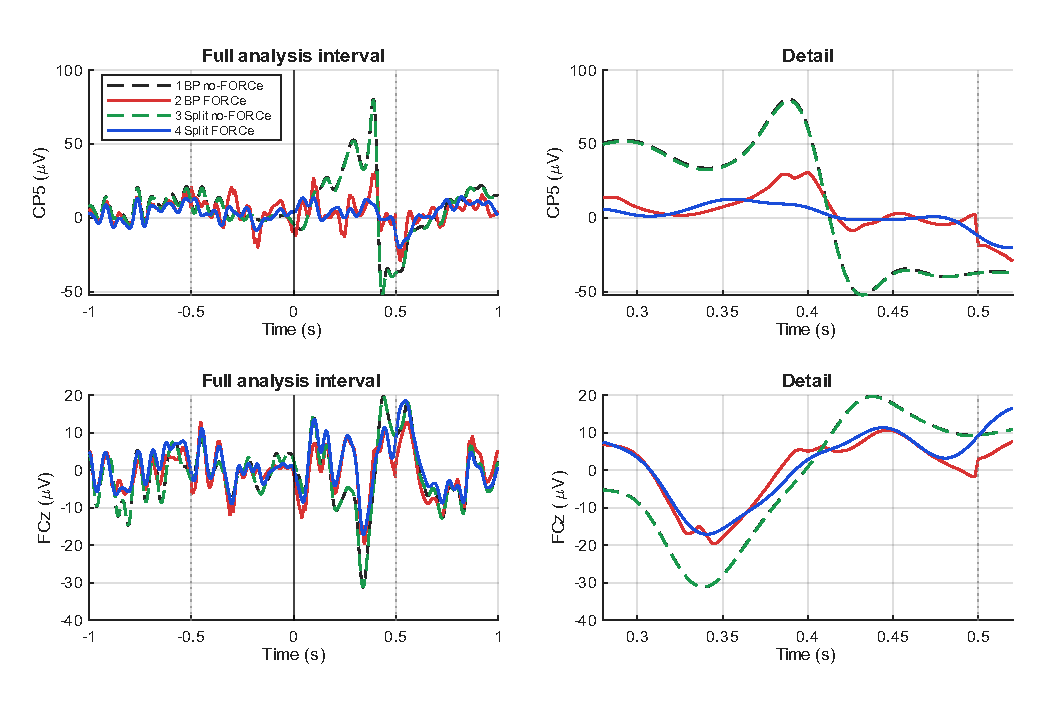
\includegraphics[width=\linewidth,height=.45\textheight,keepaspectratio]{figures/priority_3.pdf}\caption{Final outputs for spe30 / retest / run 5 / trial 80. Conditions follow Table~\ref{tab:conditions}; onset is black and cleaning joins grey dotted.}\end{figure}
\reviewbox
\clearpage
\subsection*{B.4 A new change at a cleaning join}
\textbf{mle01 / pre / run 1 / trial 70}

All conditions accept this input-unflagged trial. Bandpass FORCe has a 6.079 microvolt CP1 sample change exactly at +0.5 s, absent as such a join in the control. Split FORCe smooths the sharp change; waveform preservation is a separate question.
\begin{figure}[H]\centering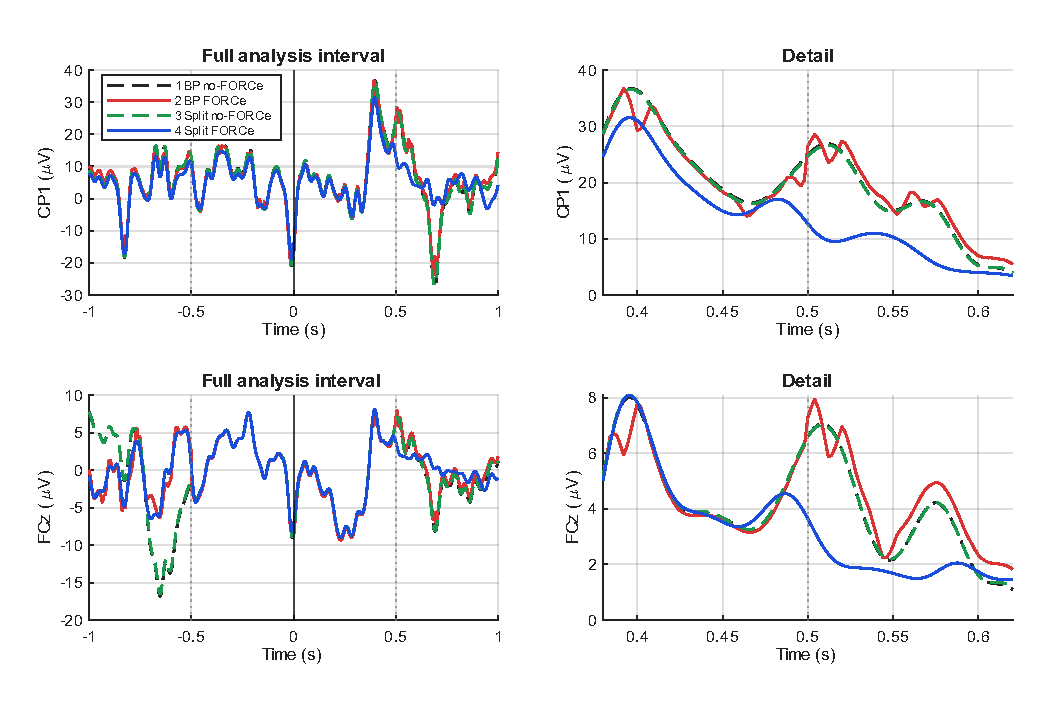
\includegraphics[width=\linewidth,height=.45\textheight,keepaspectratio]{figures/priority_4.pdf}\caption{Final outputs for mle01 / pre / run 1 / trial 70. Conditions follow Table~\ref{tab:conditions}; onset is black and cleaning joins grey dotted.}\end{figure}
\reviewbox
\clearpage\section{Matched eight-channel waveform comparisons}\label{app:erp}
\subsection*{mle01 / pre: channels 1--4}
Correct (non-displaced): $n=309$; Error (displaced): $n=166$. All outputs use identical trials.
\begin{figure}[H]\centering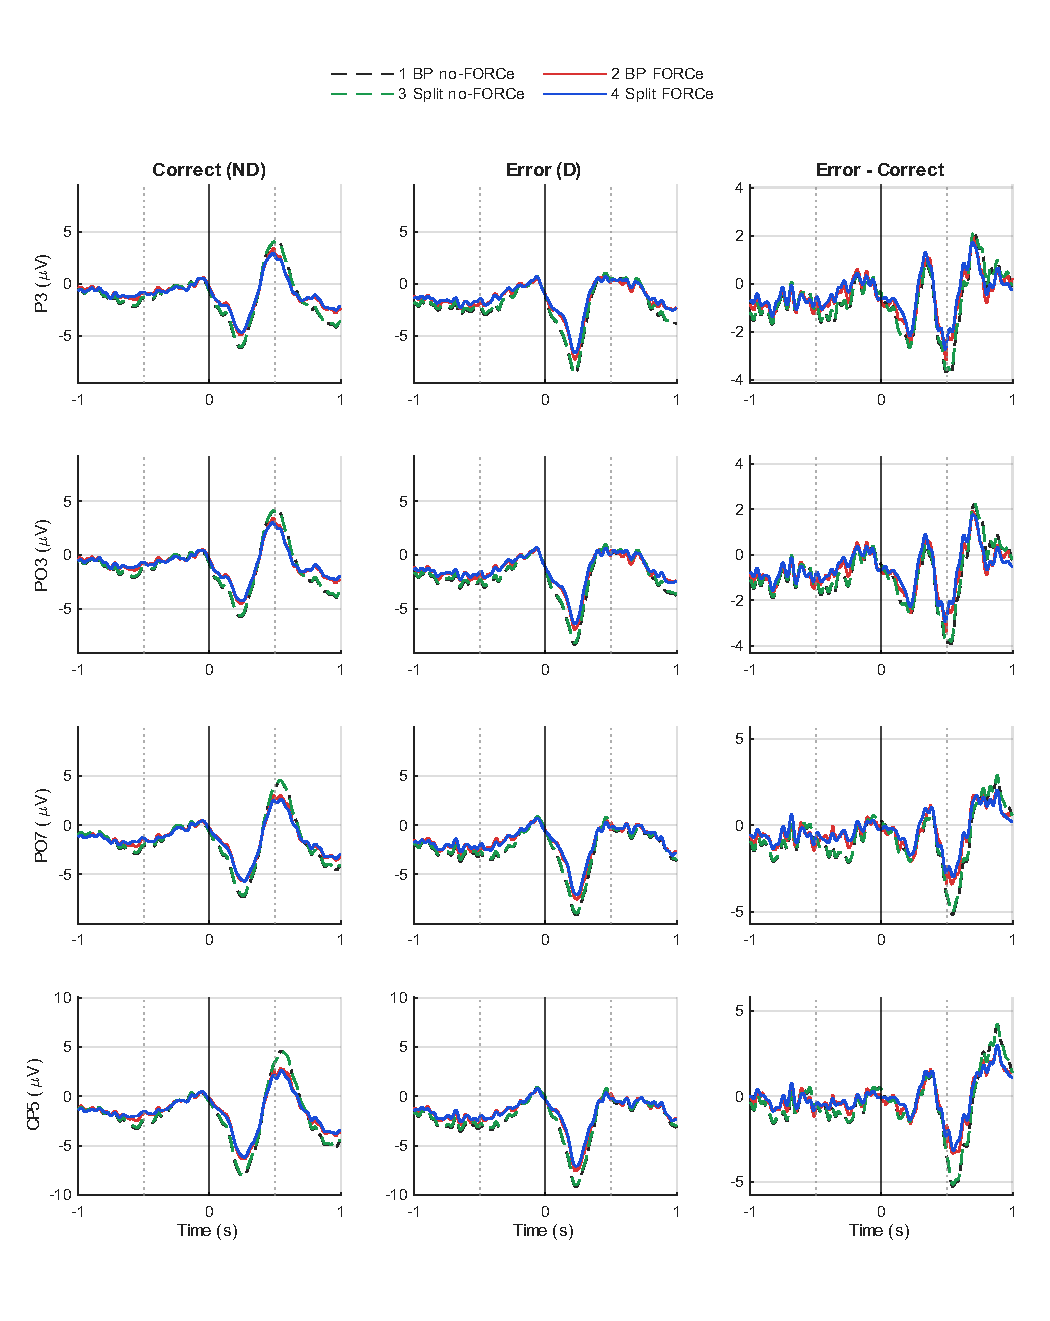
\includegraphics[width=\linewidth,height=.74\textheight,keepaspectratio]{figures/mle01_pre_group1.pdf}\caption{mle01, pre: P3, PO3, PO7 and CP5. Columns show Correct, Error and Error--Correct. Controls are dashed, FORCe solid. Onset is 0 s; joins are $\pm0.5$ s. Correct/Error share the voltage scale per channel; the difference has its own scale. Baseline: $[-0.2,0)$ s.}\end{figure}
\clearpage
\subsection*{mle01 / pre: channels 5--8}
Correct (non-displaced): $n=309$; Error (displaced): $n=166$. All outputs use identical trials.
\begin{figure}[H]\centering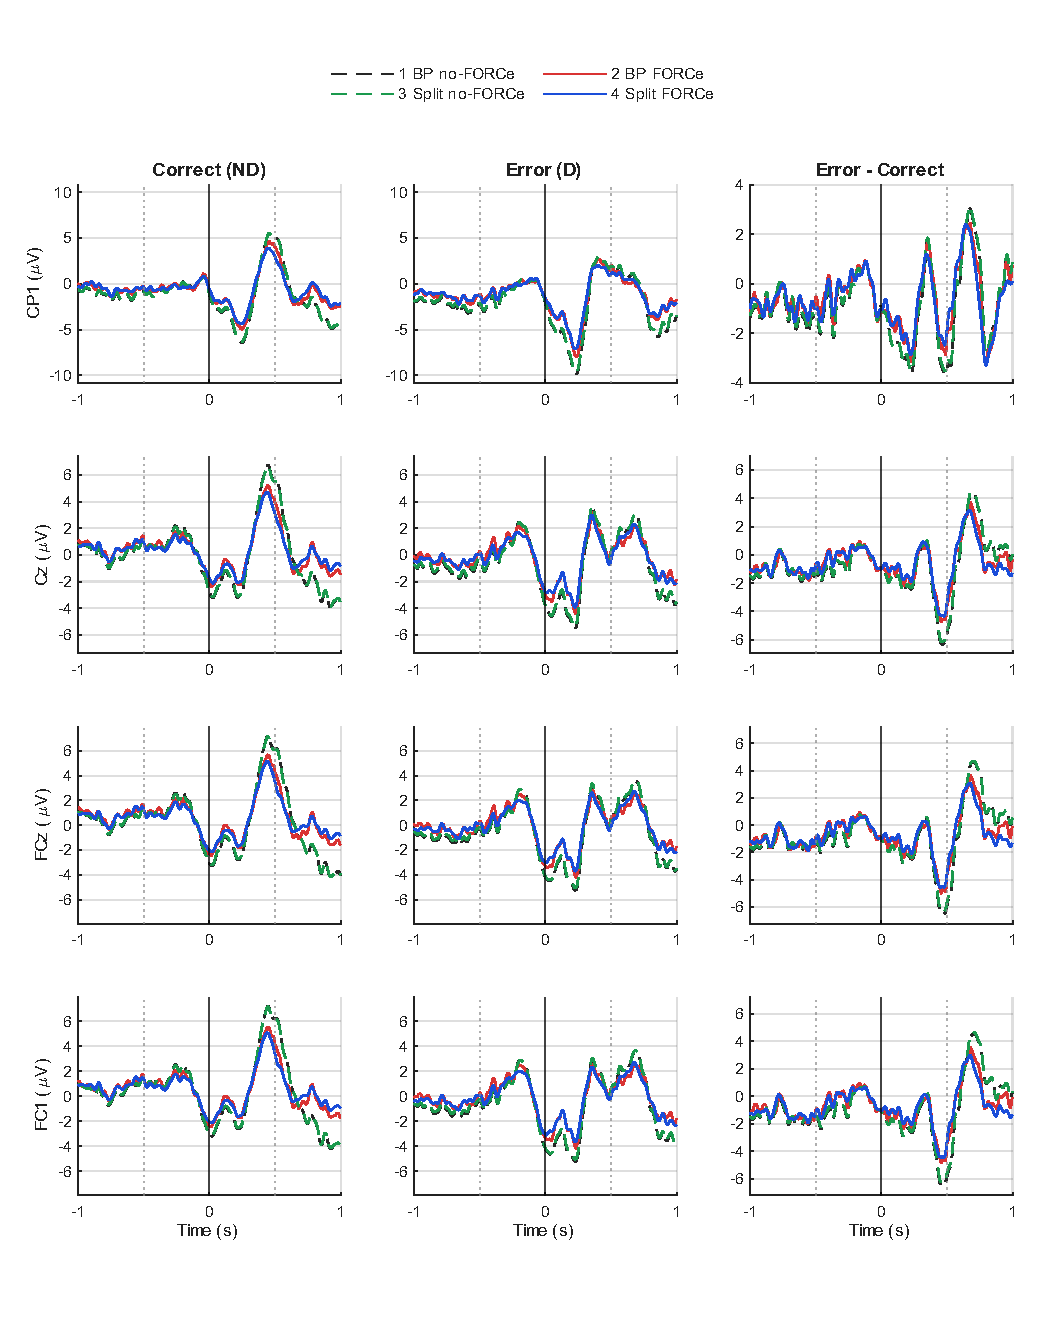
\includegraphics[width=\linewidth,height=.74\textheight,keepaspectratio]{figures/mle01_pre_group2.pdf}\caption{mle01, pre: CP1, Cz, FCz and FC1. Columns show Correct, Error and Error--Correct. Controls are dashed, FORCe solid. Onset is 0 s; joins are $\pm0.5$ s. Correct/Error share the voltage scale per channel; the difference has its own scale. Baseline: $[-0.2,0)$ s.}\end{figure}
\clearpage
\subsection*{mle01 / post: channels 1--4}
Correct (non-displaced): $n=218$; Error (displaced): $n=114$. All outputs use identical trials.
\begin{figure}[H]\centering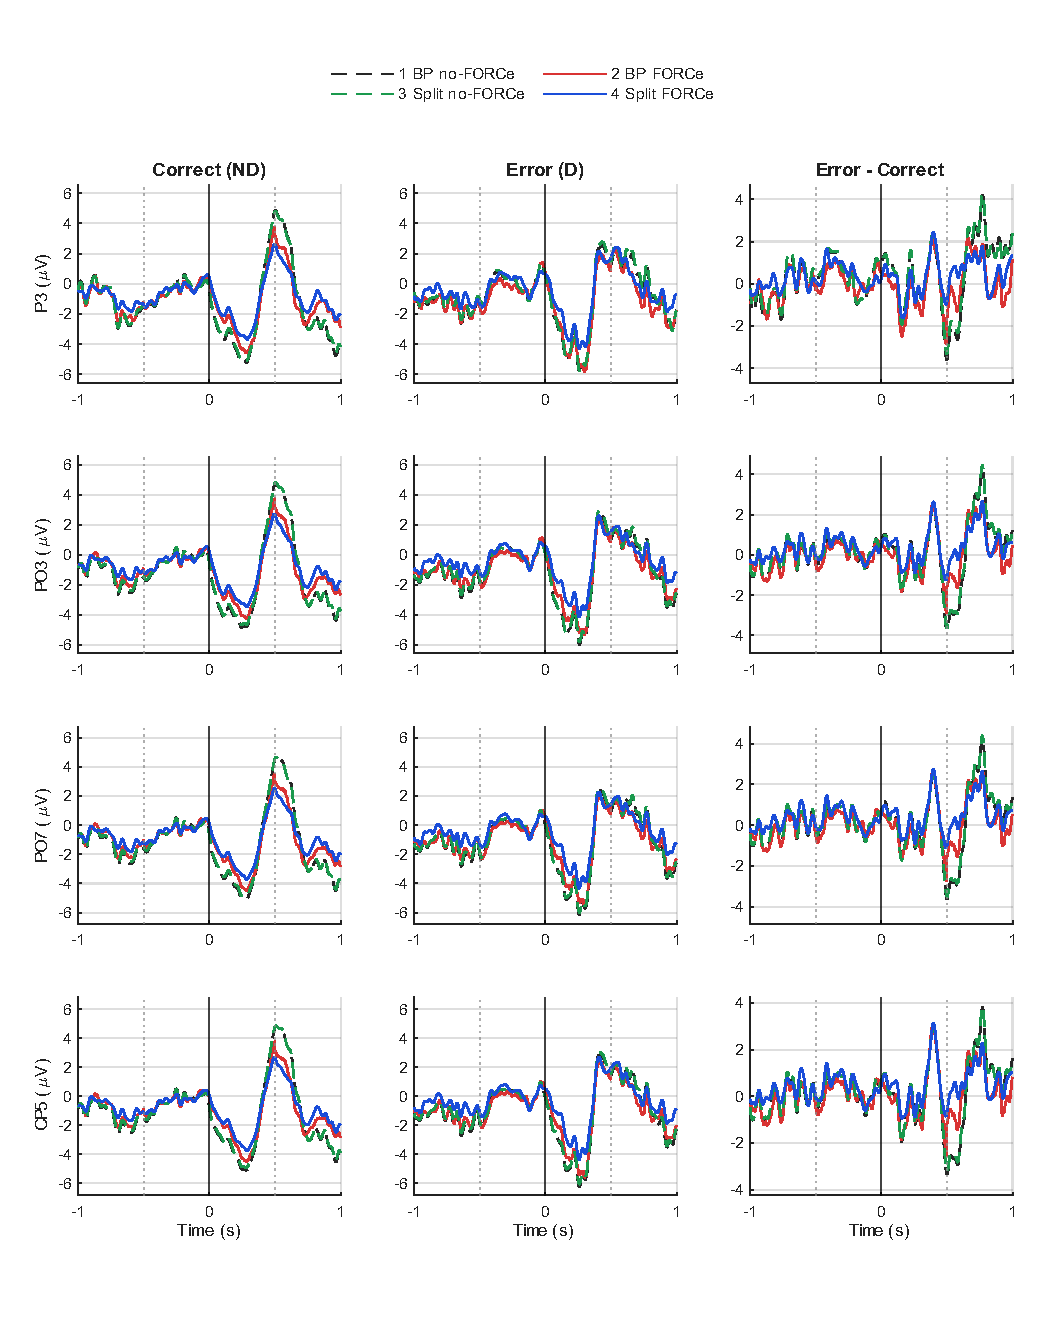
\includegraphics[width=\linewidth,height=.74\textheight,keepaspectratio]{figures/mle01_post_group1.pdf}\caption{mle01, post: P3, PO3, PO7 and CP5. Columns show Correct, Error and Error--Correct. Controls are dashed, FORCe solid. Onset is 0 s; joins are $\pm0.5$ s. Correct/Error share the voltage scale per channel; the difference has its own scale. Baseline: $[-0.2,0)$ s.}\end{figure}
\clearpage
\subsection*{mle01 / post: channels 5--8}
Correct (non-displaced): $n=218$; Error (displaced): $n=114$. All outputs use identical trials.
\begin{figure}[H]\centering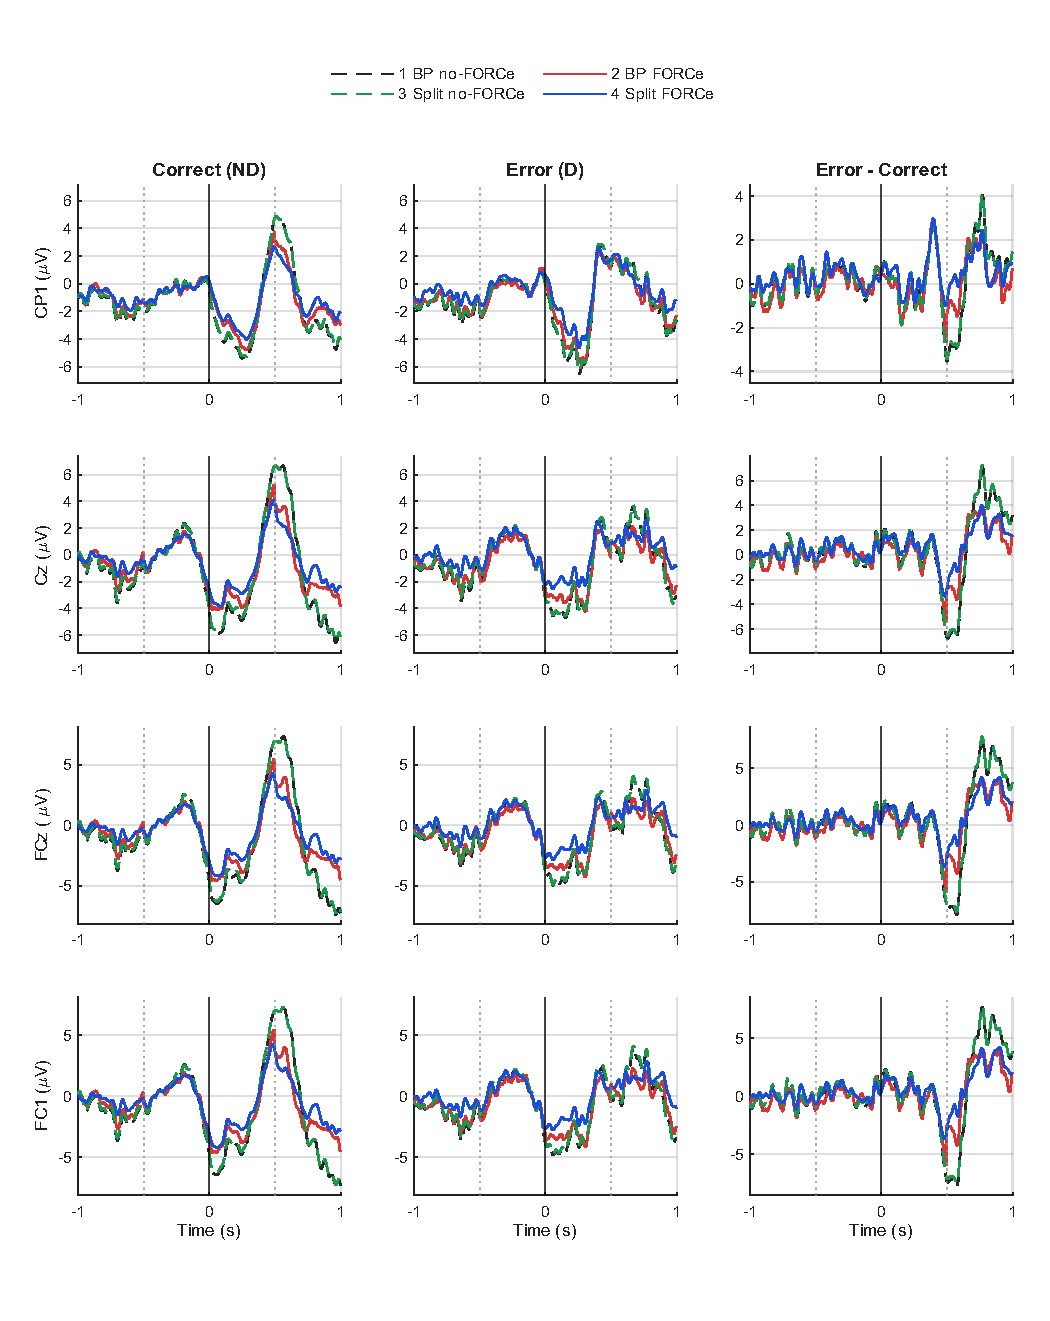
\includegraphics[width=\linewidth,height=.74\textheight,keepaspectratio]{figures/mle01_post_group2.pdf}\caption{mle01, post: CP1, Cz, FCz and FC1. Columns show Correct, Error and Error--Correct. Controls are dashed, FORCe solid. Onset is 0 s; joins are $\pm0.5$ s. Correct/Error share the voltage scale per channel; the difference has its own scale. Baseline: $[-0.2,0)$ s.}\end{figure}
\clearpage
\subsection*{mle01 / retest: channels 1--4}
Correct (non-displaced): $n=237$; Error (displaced): $n=132$. All outputs use identical trials.
\begin{figure}[H]\centering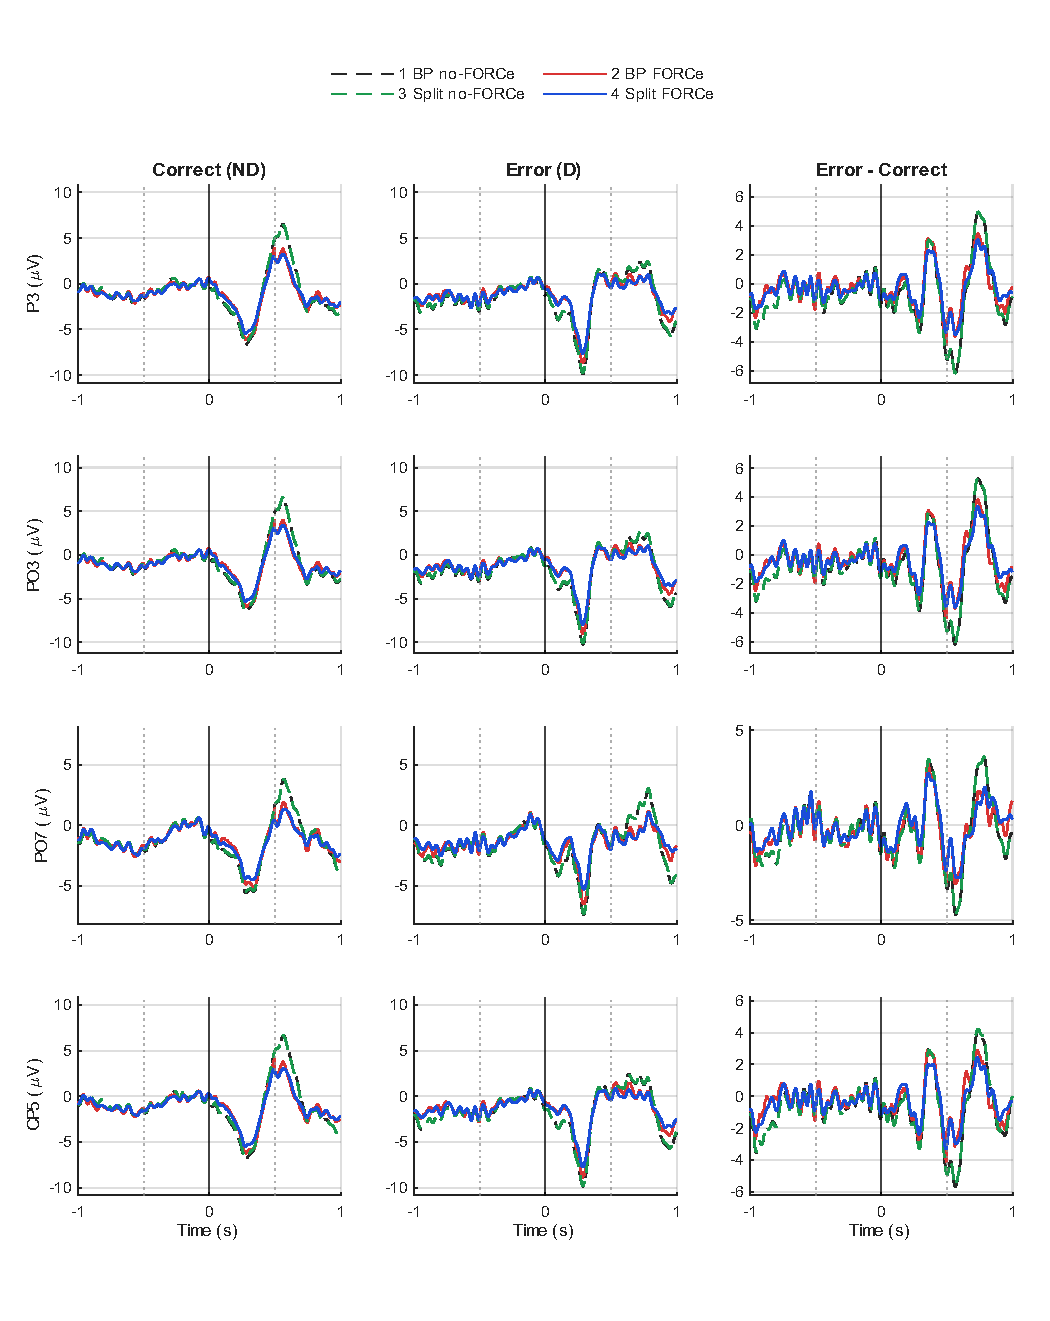
\includegraphics[width=\linewidth,height=.74\textheight,keepaspectratio]{figures/mle01_retest_group1.pdf}\caption{mle01, retest: P3, PO3, PO7 and CP5. Columns show Correct, Error and Error--Correct. Controls are dashed, FORCe solid. Onset is 0 s; joins are $\pm0.5$ s. Correct/Error share the voltage scale per channel; the difference has its own scale. Baseline: $[-0.2,0)$ s.}\end{figure}
\clearpage
\subsection*{mle01 / retest: channels 5--8}
Correct (non-displaced): $n=237$; Error (displaced): $n=132$. All outputs use identical trials.
\begin{figure}[H]\centering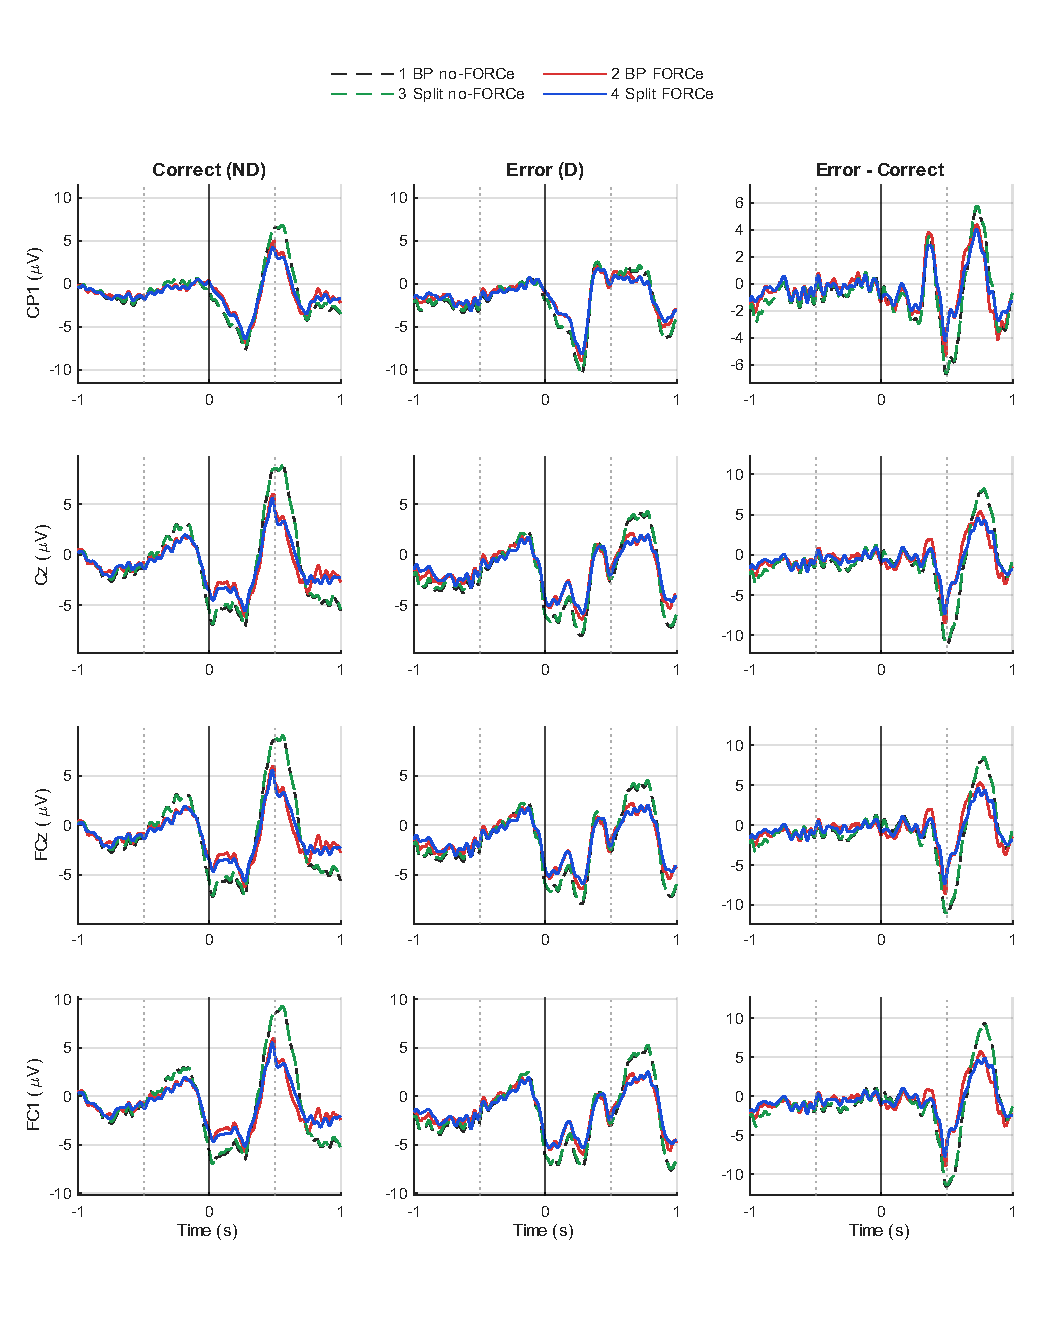
\includegraphics[width=\linewidth,height=.74\textheight,keepaspectratio]{figures/mle01_retest_group2.pdf}\caption{mle01, retest: CP1, Cz, FCz and FC1. Columns show Correct, Error and Error--Correct. Controls are dashed, FORCe solid. Onset is 0 s; joins are $\pm0.5$ s. Correct/Error share the voltage scale per channel; the difference has its own scale. Baseline: $[-0.2,0)$ s.}\end{figure}
\clearpage
\subsection*{spe30 / pre: channels 1--4}
Correct (non-displaced): $n=326$; Error (displaced): $n=169$. All outputs use identical trials.
\begin{figure}[H]\centering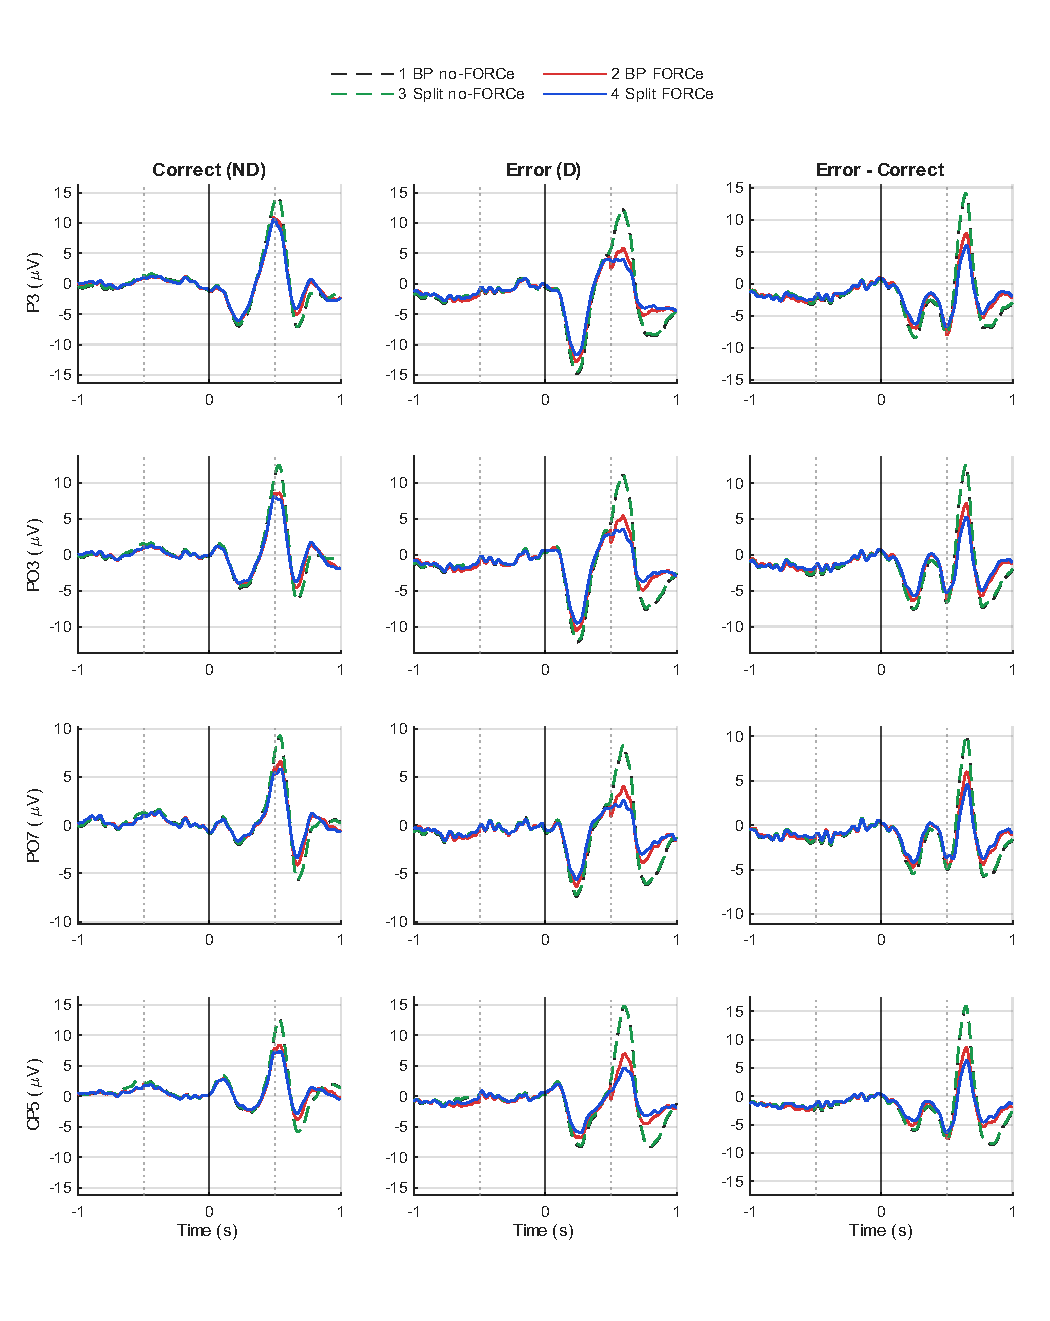
\includegraphics[width=\linewidth,height=.74\textheight,keepaspectratio]{figures/spe30_pre_group1.pdf}\caption{spe30, pre: P3, PO3, PO7 and CP5. Columns show Correct, Error and Error--Correct. Controls are dashed, FORCe solid. Onset is 0 s; joins are $\pm0.5$ s. Correct/Error share the voltage scale per channel; the difference has its own scale. Baseline: $[-0.2,0)$ s.}\end{figure}
\clearpage
\subsection*{spe30 / pre: channels 5--8}
Correct (non-displaced): $n=326$; Error (displaced): $n=169$. All outputs use identical trials.
\begin{figure}[H]\centering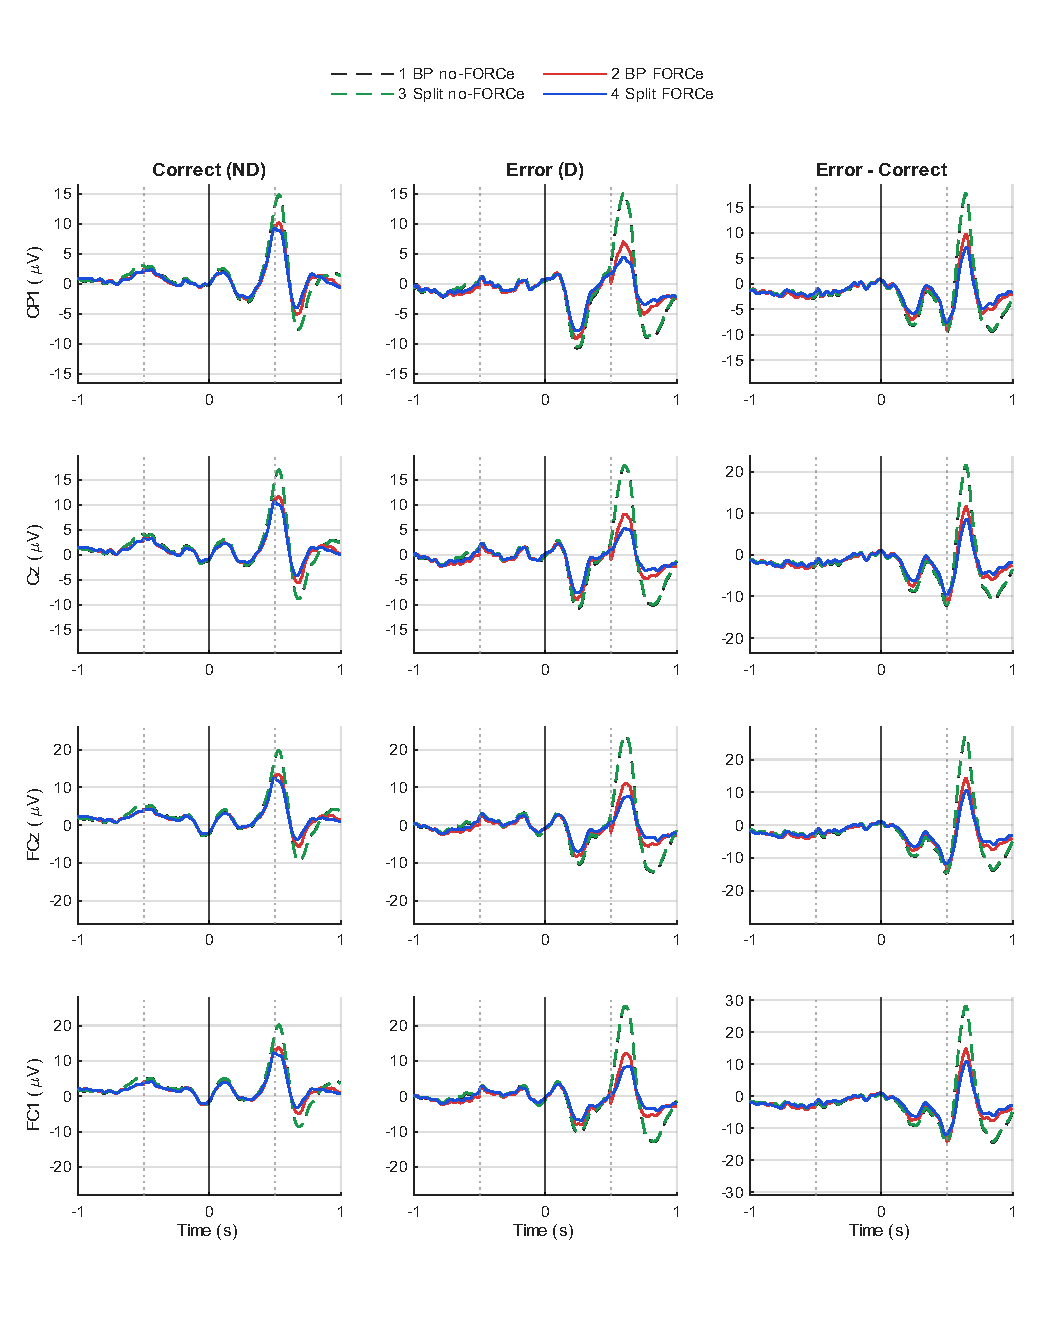
\includegraphics[width=\linewidth,height=.74\textheight,keepaspectratio]{figures/spe30_pre_group2.pdf}\caption{spe30, pre: CP1, Cz, FCz and FC1. Columns show Correct, Error and Error--Correct. Controls are dashed, FORCe solid. Onset is 0 s; joins are $\pm0.5$ s. Correct/Error share the voltage scale per channel; the difference has its own scale. Baseline: $[-0.2,0)$ s.}\end{figure}
\clearpage
\subsection*{spe30 / post: channels 1--4}
Correct (non-displaced): $n=329$; Error (displaced): $n=169$. All outputs use identical trials.
\begin{figure}[H]\centering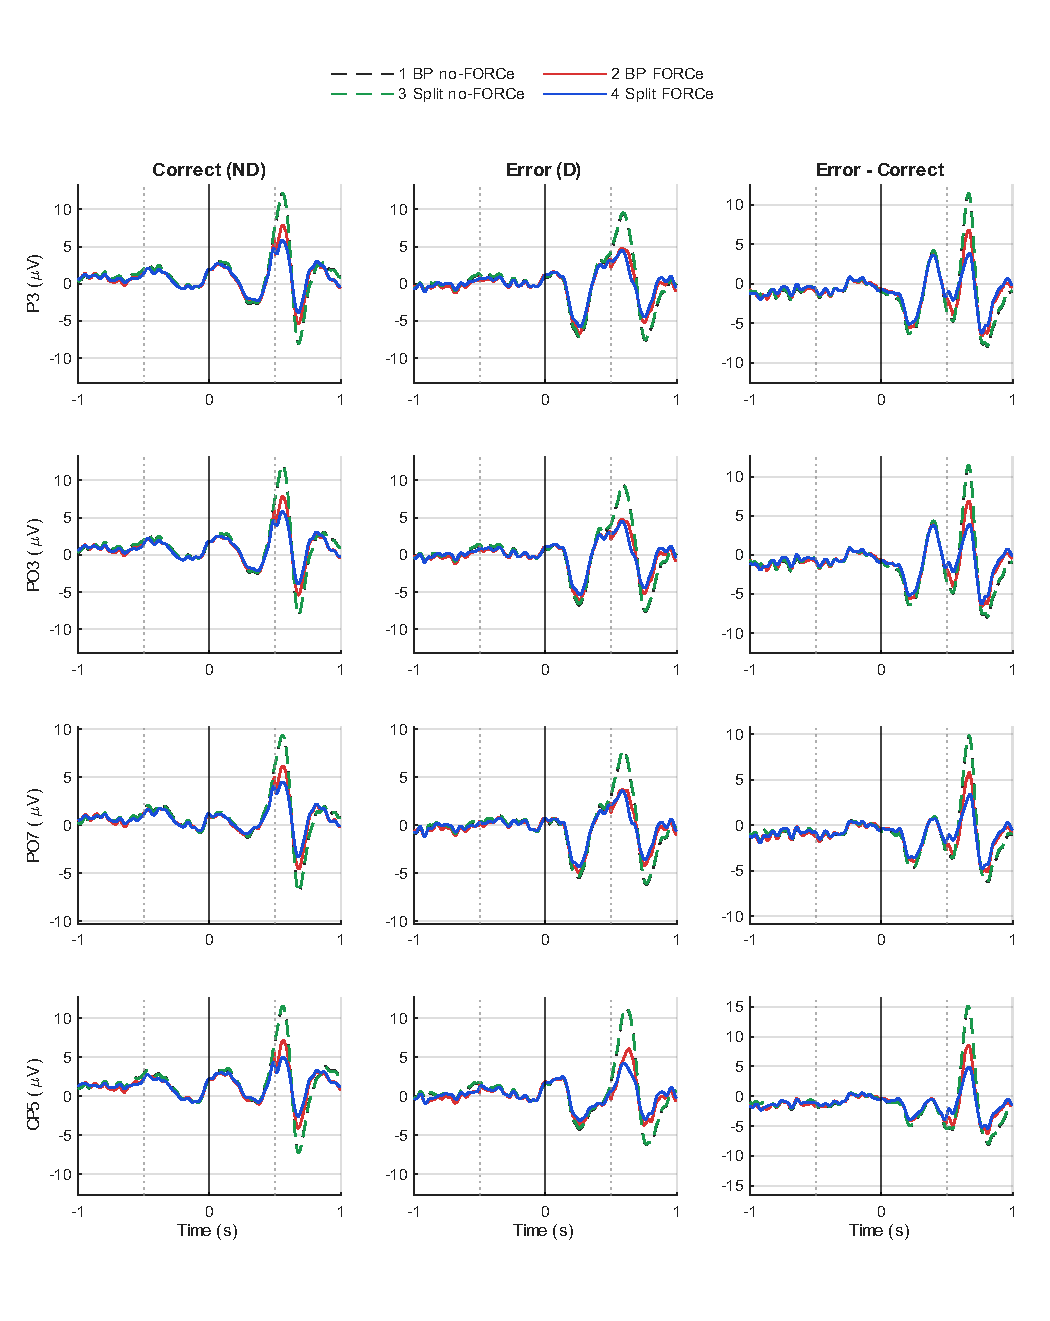
\includegraphics[width=\linewidth,height=.74\textheight,keepaspectratio]{figures/spe30_post_group1.pdf}\caption{spe30, post: P3, PO3, PO7 and CP5. Columns show Correct, Error and Error--Correct. Controls are dashed, FORCe solid. Onset is 0 s; joins are $\pm0.5$ s. Correct/Error share the voltage scale per channel; the difference has its own scale. Baseline: $[-0.2,0)$ s.}\end{figure}
\clearpage
\subsection*{spe30 / post: channels 5--8}
Correct (non-displaced): $n=329$; Error (displaced): $n=169$. All outputs use identical trials.
\begin{figure}[H]\centering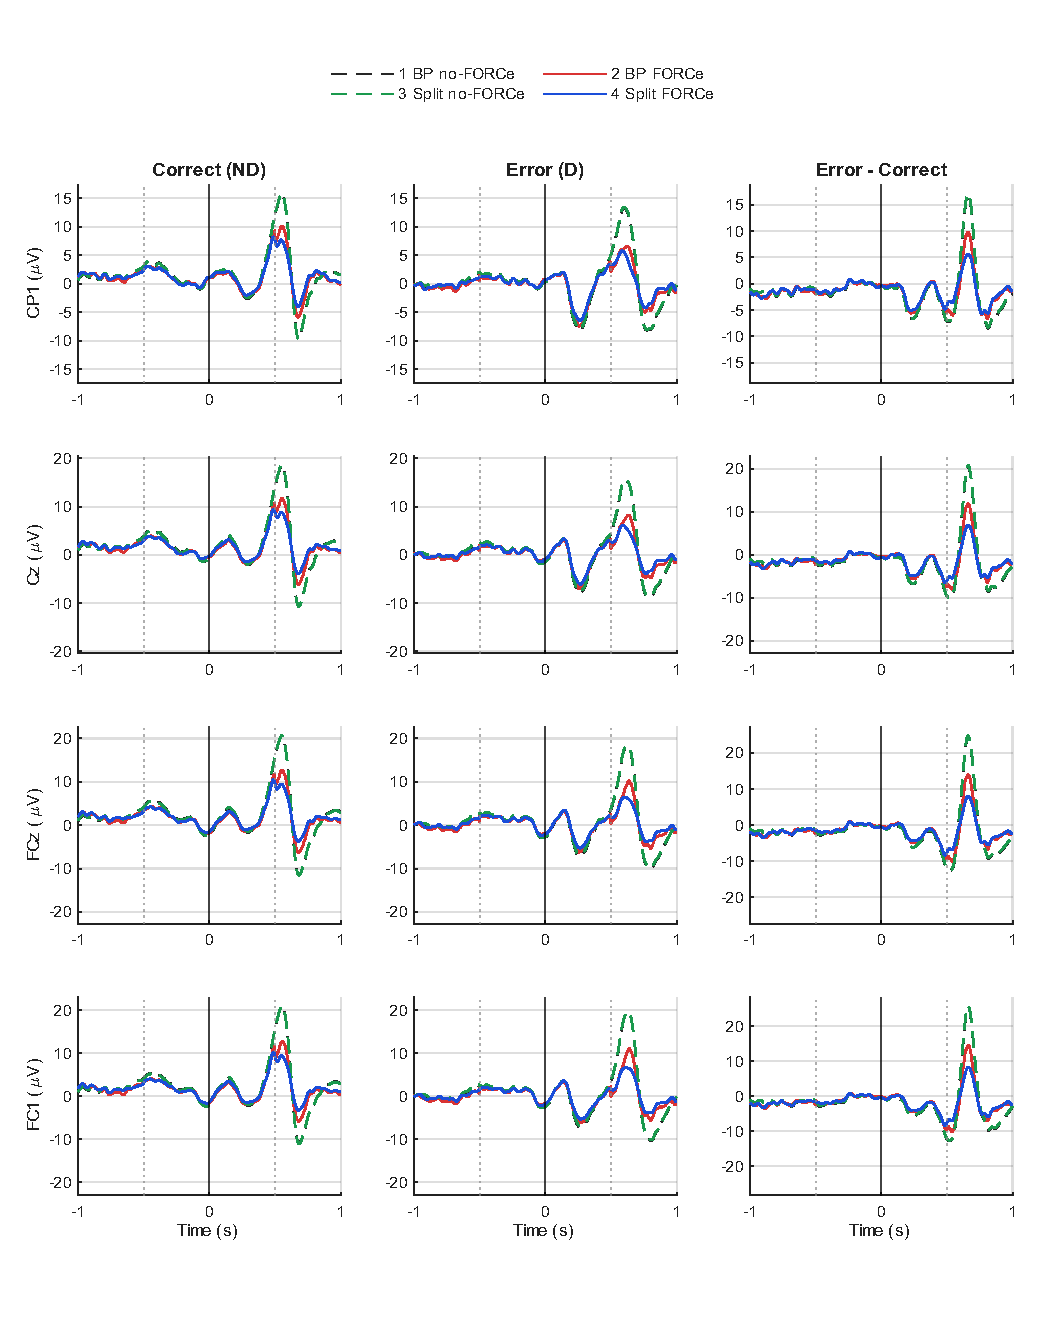
\includegraphics[width=\linewidth,height=.74\textheight,keepaspectratio]{figures/spe30_post_group2.pdf}\caption{spe30, post: CP1, Cz, FCz and FC1. Columns show Correct, Error and Error--Correct. Controls are dashed, FORCe solid. Onset is 0 s; joins are $\pm0.5$ s. Correct/Error share the voltage scale per channel; the difference has its own scale. Baseline: $[-0.2,0)$ s.}\end{figure}
\clearpage
\subsection*{spe30 / retest: channels 1--4}
Correct (non-displaced): $n=260$; Error (displaced): $n=133$. All outputs use identical trials.
\begin{figure}[H]\centering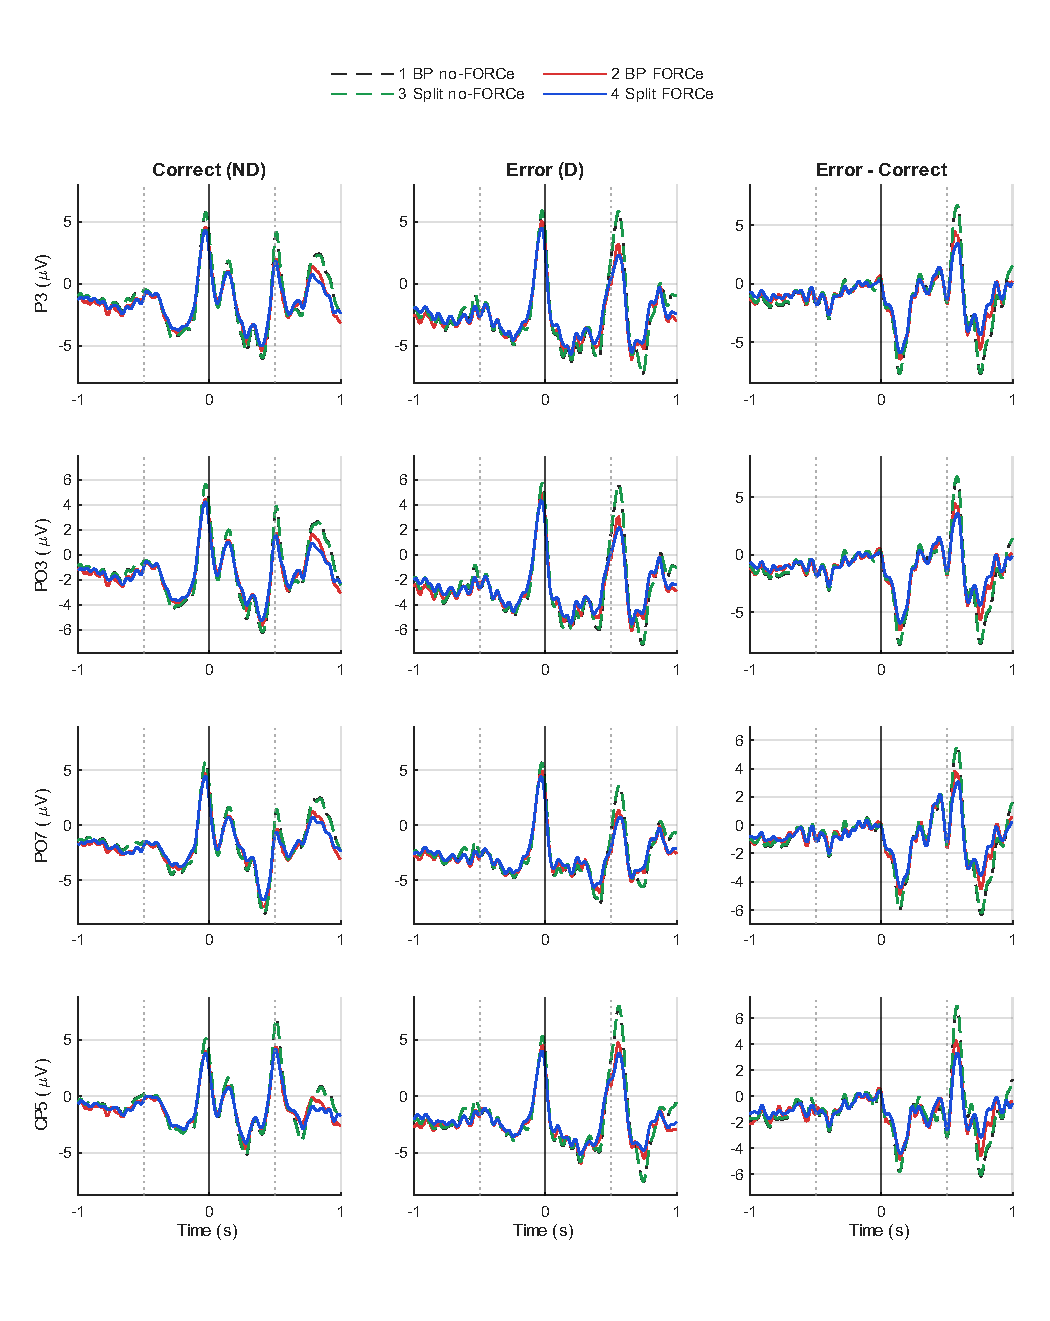
\includegraphics[width=\linewidth,height=.74\textheight,keepaspectratio]{figures/spe30_retest_group1.pdf}\caption{spe30, retest: P3, PO3, PO7 and CP5. Columns show Correct, Error and Error--Correct. Controls are dashed, FORCe solid. Onset is 0 s; joins are $\pm0.5$ s. Correct/Error share the voltage scale per channel; the difference has its own scale. Baseline: $[-0.2,0)$ s.}\end{figure}
\clearpage
\subsection*{spe30 / retest: channels 5--8}
Correct (non-displaced): $n=260$; Error (displaced): $n=133$. All outputs use identical trials.
\begin{figure}[H]\centering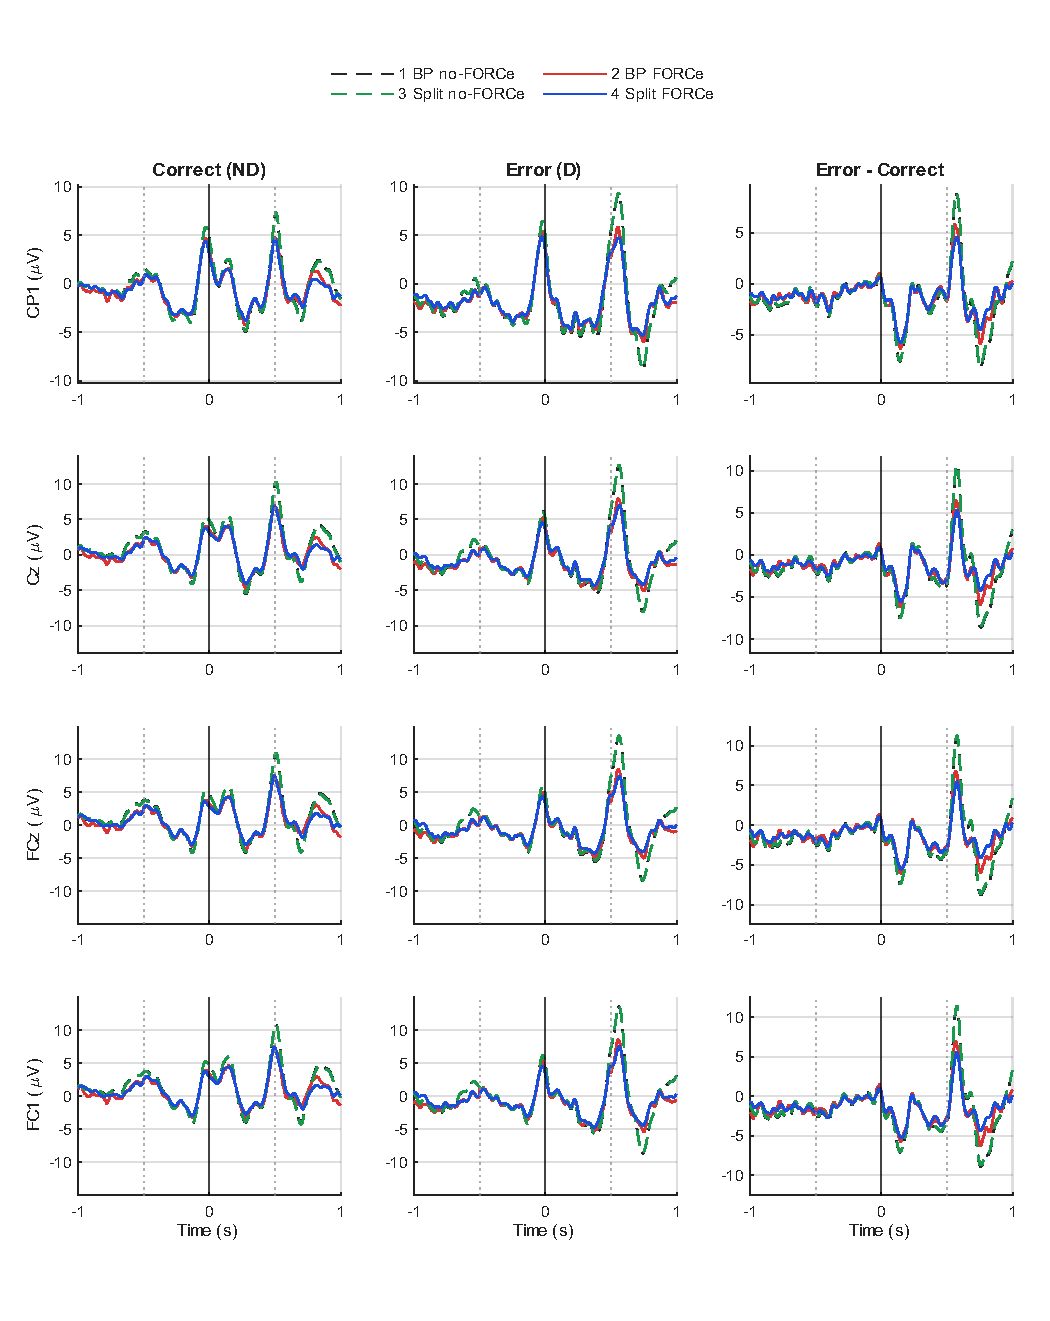
\includegraphics[width=\linewidth,height=.74\textheight,keepaspectratio]{figures/spe30_retest_group2.pdf}\caption{spe30, retest: CP1, Cz, FCz and FC1. Columns show Correct, Error and Error--Correct. Controls are dashed, FORCe solid. Onset is 0 s; joins are $\pm0.5$ s. Correct/Error share the voltage scale per channel; the difference has its own scale. Baseline: $[-0.2,0)$ s.}\end{figure}
\end{document}
